% Couverture MFA des 10 comptes privilégiés de l'export (T03, T04)
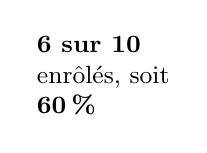
\begin{tikzpicture}[font=\scriptsize]
  \foreach \cpt/\m [count=\i from 0] in \Comptes{
    \pgfmathtruncatemacro\col{mod(\i,5)}\pgfmathtruncatemacro\lig{div(\i,5)}
    \ifnum\m=1 \def\kcol{vert}\def\ktxt{MFA enrôlé}\else\def\kcol{alerte}\def\ktxt{sans MFA}\fi
    \node[draw=\kcol, fill=\kcol!12, rounded corners=2pt, minimum width=2.75cm, minimum height=0.95cm, align=center]
      at (\col*2.95,-\lig*1.15) {\textbf{\cpt}\\[-1pt]{\color{\kcol}\ktxt}};}
  \node[anchor=west, align=left, font=\small] at (14.1,-0.57) {\textbf{6 sur 10}\\ enrôlés, soit\\ \textbf{60\,\%}};
\end{tikzpicture}
